Las áreas de los cuadrados adyacentes a dos lados de un triángulo
rectángulo son 35 unidades$^2$ y 50 unidades$^2$.
\begin{figure}[H]
    \begin{center}
        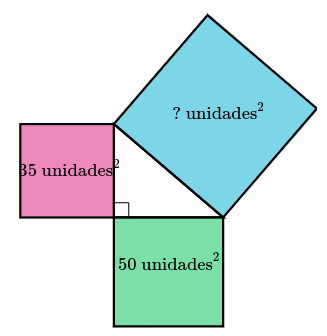
\includegraphics[width=0.4\textwidth]{../images/area4.png}
    \end{center}
    \caption{}
    \label{fig:area4}
\end{figure}
\textbf{¿Cuál es el área del cuadrado adyacente al tercer lado del triángulo?}